\chapter{2020-05-05}
\date{ }

%\begin{document}

%\maketitle
%\date{28 April, 2020}
	
	

\section{To do}

 \begin{todolist}
    \item  Experimental results
     \item  Papers about graph alignments 
    \item[\done]  Review the code for the top10 prediction 
\end{todolist}

\subsection{Code Review}
\begin{enumerate}
    \item Non-convergence $\leftarrow$swow doesn't suitable for 4 layer gcn.
         Solutions:
        \begin{todolist}
            \item[\done]    1. reduce SWOW rgcn and gcn layers
            \item    2. Information only flows from SWOW to ConcepeNet, not reverse
        \end{todolist}
        
    \item K-neighbours module has problem. Solutions:
        \begin{todolist}
            \item[\done] 1. only use top1 neighbour
            \item 2. set distance threshold
           \item 3. swap neighbours 
           \item[\done] 4. control the ratio between first rgcn and top gcn
        \end{todolist}

    \item Add alignment regularization 

    Analysis:
    The build\_nb\_graph is called in each batch. So the cross-network graph is different at each batch, which generating chaos for the node's representation. 
    Solutions:
    \begin{todolist}
    \item call build\_nb\_graph at each epoch. The advantage is that in each epoch, the model is training on a same cross-network. 
    \item Use swap neighbours method to fix the cross-network graph during whole training. (which is equa
    \end{todolist}

\end{enumerate}

\subsection{Paper Reading}
 
    \begin{todolist}
      \item[\done] survey
        \begin{itemize}
            \item  \href{https://arxiv.org/pdf/2002.00388.pdf}{A Survey on Knowledge Graphs:
Representation, Acquisition and Applications} 
            \item  \href{https://arxiv.org/pdf/2003.07743.pdf}{A Benchmarking Study of
Embedding-based Entity Alignment for Knowledge Graphs}
            \item \href{https://arxiv.org/pdf/1911.08342.pdf}{Knowledge Graph Entity Alignment with Graph
Convolutional Networks: Lessons Learned}
        \end{itemize}
      \item MultiKE: \href{https://arxiv.org/pdf/1906.02390.pdf}{Multi-view Knowledge Graph Embedding for Entity Alignment} %Swapping
      \item[\done] \href{https://arxiv.org/pdf/1911.08936.pdf }{AliNet:Knowledge Graph Alignment Network with Gated Multi-hop
Neighborhood Aggregation (AAAI 2019}    %neighbour embedding
      \item \href{https://www.ijcai.org/Proceedings/2019/0574.pdf}{A Vectorized Relational Graph Convolutional Network for Multi-Relational Network Alignment (IJCAI 2019)}  %regularization (new, and code available)
      
      \end{todolist}

\section{Summary}
\begin{enumerate}
    \item The non-convergence problem is because of two reasons: 1) the gcn layers for swow is too many, 2) the neighbors for the second gcn layer are not selected. \cite{Sun2019KnowledgeGA} also shows that with the increase of gcn layers, the MRR and HITS@N decrease a lot, seen Figure~\ref{fig:more_gcn_less_mrr}. 
    \begin{figure}[!ht]
    \centering
    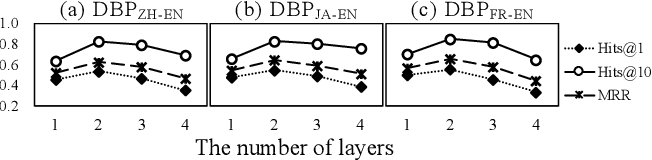
\includegraphics[scale=0.5]{images/0505/6-Figure4-1.png}
    \caption{With the increase of GCN layers, the MRR decreases a lot. From \cite{Sun2019KnowledgeGA}}
    \label{fig:more_gcn_less_mrr}
    \end{figure}

     \item About the neighbourhood selection 
      From the view of graph dendification. About graph densification, two kind of methods have been used.  \\
         1)  \textbf{Add training data explicitly}
         \begin{itemize}
             \item \textbf{Hard Selection}: Based on the assumption that an aligned pair of nodes should have similar neighbors in two kgs, some studies \citep{Ye2019AVR,Hu2019MultiKEAM,Zhu2019NeighborhoodAwareAR} 
        on graph alignment adopt the neighborhood swapping method to exchange the neighbors for aligned seed entities, and then add these generated triples back to the original graphs.  \\
        \item \textbf{Hard\&Soft}:
        \cite{Malaviya2019ExploitingSA} generate more training triplets by 1): selecting nodes with high similarities using the node's representations from a pre-trained BERT model, 2) adding reverse edges for all triples (directed graph directed graph $\rightarrow$  undirected graph). 
        Similarly, by arguing that distant (multi-hop) neighbors can also contribute to the entity alignment, \cite{Sun2019KnowledgeGA} allow distant neighbors together with direct neighbors (one-hop) to directly update the centered node representation. They use a gated mechanism to decide the importance of the distance neighbours and the direct neighbours. 
        \item{Rule-based} 
         MuGNN \citep{cao-etal-2019-multi} is the first paper I have read that jointly train KG completion and entity alignment. However, their completion module is based on rules, and they add margin loss to distinguish rule grounded triples and negative triples. 
         
        %现在的enetity alignment work ignored the heterogeneous structure problem. the core idea of this paper is generate similar structure for two nodes in two graphs by add missing edges and pruning irrelevant edges. It's the first I read that jointly train KG completion and entity alignment\\
        
    \end{itemize}
         2) \textbf{Cross-KG representation augmentation} \\
         For entities having fewer same neighbours in two graphs, GMNN \citep{xu-etal-2019-cross-lingual} claim that utilizing bilingual structure is better than monolingual structure information and thus formulate the problem of entity alignment as a graph matching problem by borrowing the idea from sequence matching. The bilingual representation is the concatenation of the original graph representation from a GCN and cross-KG attentive graph representation from its counterpart graph. \\
        This also can be seen as a kind of graph densification. 
        So basically, there are two options for the source of candidate neighbors: the original graph, and the another graph. So far, I haven't seen any papers combining both of them. 
           %\begin{table}[!h]
           %     \centering
           %     \begin{tabular}{c|c|c|c|c|c}
           %     \hline
           %         model &  source & soft\_or\_hard & selection\_method & inject\_at\_where & how\_to\_inject\\\hline
           %          & \\
           %     \hline
           %     \end{tabular} 
           %     \caption{Caption}
           %     \label{tab:my_label}
           % \end{table}
    \item  K-nearest neighbours 
         \begin{itemize}
             \item  The similarity distance from FAISS is decreasing with the training time increasing. It's hard to set up a fixed threshold directly to cut off the unimportant. This may cause  no neighbours are selected at the beginning of training. \\ 
             One possible way could be use the original neighbours at the beginning of training, and replace the neighbours when the model is warmed up.
             \item For now, I only choose the top1 nearest neighbour. (Still needs to figure out a better way.) This caused the \textit{hubness} problem, which means a hub of ponits frequently appear as the top-1 nearest neighbors of many other points. 
                \begin{table}[!ht]
                    \centering
                    \begin{tabular}{c|cccc}
                    \hline
                         Source&graph-type & \#Nodes & \#Edges & \#Shared\_Nodes \\  \hline
                         Original-Sub& ConceptNet &  7946 & 8000 & 1601 \\
                         & SWOW & 10467 & 8000 & 1601 \\
                         \hline
                         Cross-Sub & ConceptNet & 8246 & 7946&  \\
                            & SWOW & 12153 & 10467 & \\
                         \hline
                    \end{tabular}
                    \caption{\textit{Hubness} Problem caused by top1 nearest neighbour}
                    \label{tab:my_label}
                \end{table}
            \item  \textcolor{red}{TODO}: For now, the cross-network is generated in each batch. Intuitively, I don't think it's a good idea. So, generate a cross-network at each epoch seems to be more reasonable. 
            \item Nearest sampling has been used as negative sampling strategy \citep{sun-etal-2018-BootEa, cao-etal-2019-multi}. And negative samples are re-calculated every N epochs. 
         \end{itemize}
        
    
    \item About the alignment supervision \\
        Assumption: ``The assumption is that entities and their counterparts in different KGs should have similar structures and thus similar embeddings."
        \begin{itemize}
            \item Use $\gamma$ to control the ratio of alignment loss term. (The jointly loss has to be carefully balanced. $\leftarrow$ heterogeneous structure) 
            \item Distance inputs, project two embeddings to a shared space or not, $distance= f(Wa,Wb)$ , $distance=f(Wa,b)$ , $distance=f(Wa,b)$ or $distance=f(a,b)$, where $f$ could be L1 or L2 norm. 
            \item How to do negative sampling $(a,b)$ $a^{\prime}, b$ $a, b^{\prime}$ $a^{\prime}, b^{\prime}$
            \item \textcolor{red}{TODO}: Where to add the alignment loss? At the batch aligned entities or on the sub-graph aligned entities. (This may be a problem of my code, I add the sub-graph alignment loss on each batch training, that may influence triples not used in current training batch. I need to modify)
        \end{itemize}
\end{enumerate}


\section{Details about graph alignments }
Alignment supervision methods:
\begin{enumerate}
    \item Swap neighbors based on aligned entity seeds to generate more triples (More training data)  
    \item Minimize the distance between the aligned pairs and increase the distance between un-aligned pairs.  (Loss Function) \\
    AVR-GCN\citep{Ye2019AVR} combines both swapping and distance regularization and by splitting the aligned entities into two parts. 
\end{enumerate}

\noindent \textbf{Alignment}
maps entities into a unified representation space under
a joint embedding framework through aligned
translation as: 
    \begin{enumerate}
        \item aligned translation$\big |\big| e_1 + r^{(E1 \rightarrow E2)}  -  e_2 \big |\big|$   
        \item linear transformation as $M^{(E1\rightarrow E2)}e_1 - e_2$    
        \item parameter sharing as $e_1 \equiv e_2$.   
        \item parameter swapping: swaps seed entities in their triples to generate extra triples as supervision, $(e_1,r,e_2) \in \mathcal{G}_1$ $(e_1,r,e_2) \in \mathcal{G}_2$ 
    \end{enumerate}
    
    
\noindent\textbf{Distance Measure methods:}
\begin{align}
    & Manhattan: \big |\big|x -y \big |\big|_{L1} = \sum_{i=1}^{n} |x_i-y_i| \\
    & Euclidean:  \big |\big|x -y \big |\big|_{L2} = \sqrt{\sum\limits_{i=1}^{n} (x_i - y_i)^2} \\
    & Cosine(x,y) =  \frac{\sum_{i=1}^{n}x_i*y_i}{\sqrt{\sum_{i=1}^{n}{x_i}^2} \times \sqrt{\sum_{i=1}^{n}{y_i}^2}}  
\end{align}

%\textbf{Loss Function}


%\begin{comment}
\section{Details that may matter}

What's the key problem I am trying to solve?  \\
1. ConceptNet is sparse. So it's necessary to introduce some densification strategies to augment nodes with more neighbors?\\
2. The overlapping between ConceptNet and SWOW is small. If we are going to learn them jointly and allow more information flow from SWOW to ConceptNet, we need them to be tied deeper. 


How to pick neighbors for cross-network graph? Or how to generate cross-network?
 1. Generate dynamic cross-network graph.
 Where to train the cross-network graph? 
 Should we generate two cross-network graphs or only one?
 2. Swap neighbours of original two kgs for aligned entities.  
 
How to make use of aligned entities as supervision signals? 

%\end{comment}



\section{TopK Prediction Observation}
\begin{figure}[!ht]
    \centering
    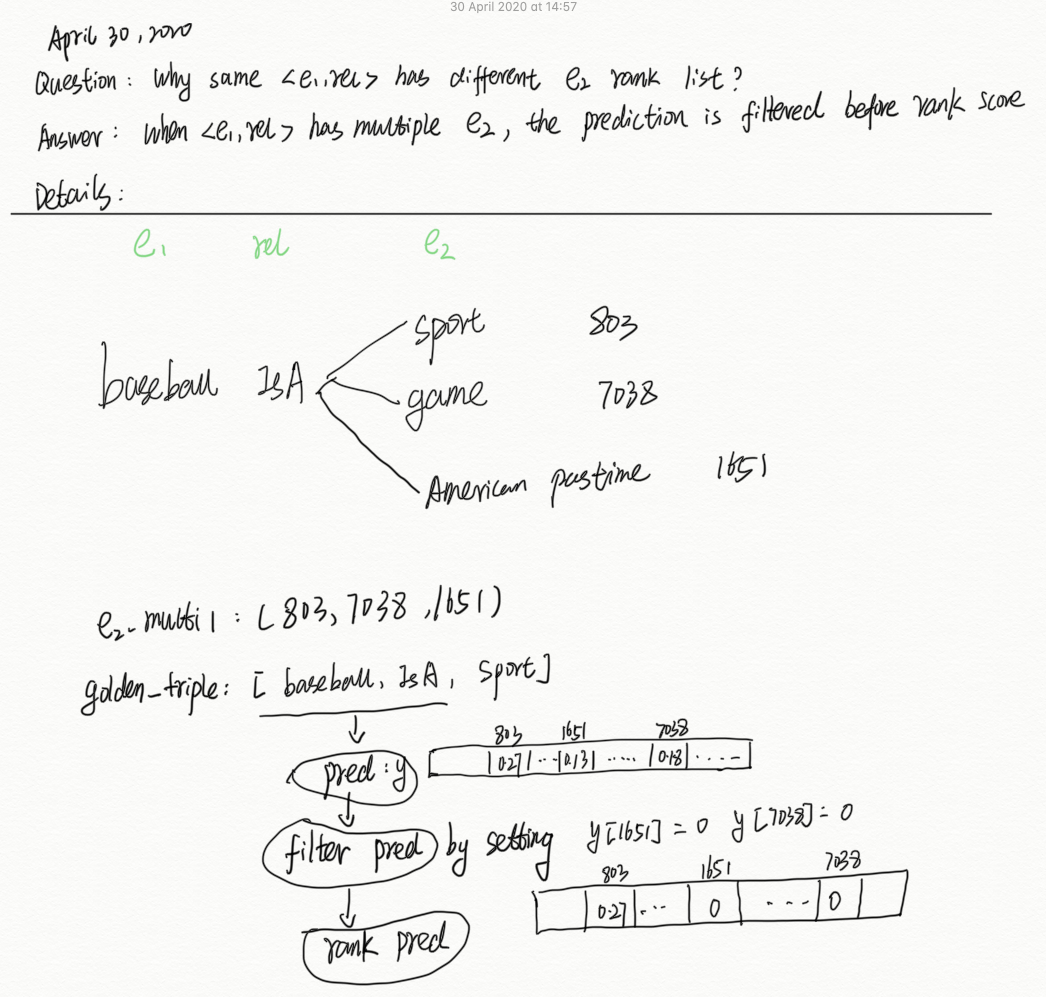
\includegraphics[width=\textwidth]{images/filter_prediction.png}
    \caption{Filter prediction before rank}
    \label{fig:my_filter_prediction}
\end{figure}

Lea: 
Yes, but why do you set "game" and "american passtime" to zero when evaluating [baseball, isA, sport]?

Chunhua: 
They say they follow the previous work. This is an updated version for compute MRR and HITS@N directly. For example, when we are evaluating the <baseball, IsA, sport> , if the score <baseball, IsA, game> is higher than the <baseball, IsA, sport>, then when computing the loss, the model would think this is a wrong prediction. But actually, it’s true. 

Originally from \href{https://papers.nips.cc/paper/5071-translating-embeddings-for-modeling-multi-relational-data.pdf}{Translating Embeddings for Modeling Multi-relational Data}


%\printbibliography
%\end{document}


